% 1977 年山东B卷第 6 题：正四棱锥的二视图（按源卷第 2 页布局）
% 上：正面图（三角形，垂直点划中心线）；下：俯视图（正方形加两条对角线，十字中心线）
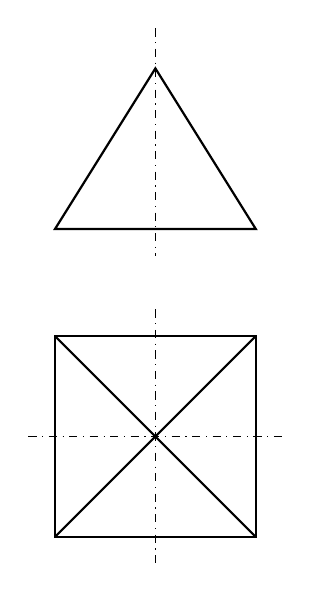
\begin{tikzpicture}[scale=0.85]
  % ---- 正面图：三角形 ----
  \coordinate (apex) at (0,2.4);
  \coordinate (bl) at (-1.5,0);
  \coordinate (br) at (1.5,0);
  \draw[thick] (bl)--(apex)--(br)--cycle;
  % 正面图垂直中心线（点划线，超出图形）
  \draw[dash dot] (0,3.0)--(0,-0.4);
  % ---- 俯视图：正方形 + 对角线 ----
  \coordinate (s1) at (-1.5,-1.6);
  \coordinate (s2) at (1.5,-1.6);
  \coordinate (s3) at (1.5,-4.6);
  \coordinate (s4) at (-1.5,-4.6);
  \draw[thick] (s1)--(s2)--(s3)--(s4)--cycle;
  \draw[thick] (s1)--(s3);
  \draw[thick] (s2)--(s4);
  % 俯视图十字中心线（点划线，超出图形）
  \draw[dash dot] (0,-1.2)--(0,-5.0);
  \draw[dash dot] (-1.9,-3.1)--(1.9,-3.1);
\end{tikzpicture}
